\documentclass[a4paper,12pt, final]{report}
\usepackage{graphicx}
\usepackage{url}
\usepackage{float}
%\usepackage[nomain,acronym,xindy,toc]{glossaries} % nomain, if you define glossaries in a file, and you use \include{INP-00-glossary}
%\makeglossaries
%\usepackage[xindy]{imakeidx}
%\makeindex
%\usepackage[section]{placeins}
\renewcommand\bibname{References}
\usepackage[utf8]{inputenc}
%\usepackage{algorithm2e}
%\usepackage{wrapfig}
\usepackage{epsfig}
%\usepackage{hyperref}
\usepackage[hidelinks]{hyperref} % To Hide the box around links
\renewcommand\bibname{References}
%\usepackage{algorithm2e}
\usepackage{color}
\usepackage{textcomp}
\usepackage{acronym}
\usepackage[top=0.5in, bottom=1in, left=1in, right=1in]{geometry}
\usepackage{xcolor}
\definecolor{dark-red}{rgb}{0.4,0.15,0.15}
\definecolor{dark-blue}{rgb}{0.15,0.15,0.4}
\definecolor{medium-blue}{rgb}{0,0,0.5}

\setlength{\parskip}{0.5em}

\newcommand{\BigO}[1]{\ensuremath{\operatorname{O}\bigl(#1\bigr)}}
\parindent 8pt
\begin{document}
  \thispagestyle{empty}
  \vspace*{1cm}
  {\centering     
  \textbf{\LARGE TITLE TBD}\\
  \vspace{1.20cm}
  %\it
  %\vspace{.5cm}
  %\rm
  \textbf{\large Dual Degree Project Stage 1 Report}\\
  \vspace{1cm}
  {Submitted in partial fulfillment of the requirements}\\
  \vspace{0.25cm}
  {for the}\\
  \vspace{1cm}
  \textbf{ Dual Degree Programme}\\
  \vspace{1.50cm}
  {by}\\
  \vspace{0.20cm}
  \textbf{\large Janeel Patel}\\
  \vspace{0.25cm}
  \textbf{\large (Roll No. 180020038)}\\
  \vspace{1.8cm}
  {Under the guidance of}\\
  \vspace{0.20cm}
  \textbf{\large Prof. Virendra Singh}\\
    \vspace{0.30cm}
  \vspace{1.450cm}
    \begin{figure}[htb]
    \begin{center}
    
\includegraphics[height=1.5in,width=1.5in]{august22/img/iitblogo.png}
    \end{center}
    \end{figure}

    
  {\textbf{Department of Electrical Engineering}}\\
  {\textbf{Indian Institute of Technology Bombay}}\\
  {\textbf{August 2022}}
 
 }
 
\renewcommand{\abstractname}{Acknowledgement}
\begin{abstract}
I express my gratitude to my guide Prof. Virendra Singh for providing me the opportunity to work on this topic. I would also like to thank Mr. Rajkumar Choudhary for his invaluable time and support.
\\\\
\\\\
\\\\
Janeel Patel\\
Electrical Engineering\\
IIT Bombay\\\

\end{abstract}


\clearpage 
\renewcommand{\abstractname}{Abstract} 
\abstract{To be added.
}

\tableofcontents
  \addcontentsline{toc}{chapter}{\listfigurename}
  \listoffigures
%  \printglossaries

%\newglossaryentry{ILP}
%{name = ILP,
%description = Instruction Level Parallelism}

\chapter{Introduction}

The goal for August 2022 was to get acquainted with Sniper multi-core simulator v6.1 \cite{sniper} by understanding already existing projects and models for the Load Slice Core \cite{loadslice}, the Forward Slice Core \cite{forwardslice} and the Freeflow Core \cite{freeflow}. The aim was to also run modified versions of these implementations to develop a deeper understanding of the implemented project and the underlying research work.

\section{Background}

Processors in recent times are designed to either provide significant energy savings (in-order cores) or deliver high performance (superscalar out-of-order cores). At one end of the spectrum, we have in-order (InO) cores that are extremely energy efficient owing to their simple design, while on the other end of the spectrum, we have elaborate superscalar out-of-order (OoO) designs which are extremely power-hungry due to complex performance-boosting hardware structures. An ideal core design should provide high performance at a reasonably low power overhead.

To overcome the slow in-order execution model of InO cores, restriced OoO cores have been proposed to exploit memory hierarchy parallelism (MHP\footnote[1]{MHP is defined as the average number of overlapping memory accesses that hit anywhere in the cache hierarchy (including the main memory).}) and to improve instruction level parallelism (ILP) with respect to the standard stall-on-use InO pipeline. A stall-on-use InO pipeline is halted when an instruction that consumes an older load stalls the head of the issue queue, in case of a producer load miss. Now, depending on which cache level this miss is serviced from, the processor stalls for tens to hundreds of cycles. Younger independent instructions are thus disallowed to execute even though they are ready.

\cite{loadslice}, \cite{forwardslice}, \cite{freeflow}, all of these papers propose a restricted OoO core microarchitecture with multiple InO queues that dispatch specific kinds of instructions to each queue, and issue instructions from the queue heads. So, instructions are issued in-order from each particular queue, but out-of-order from the heads of various queues as and when instructions at the head of each queue get ready for execution.

\chapter{Literature Survey}

In this section, we go through the microarchitecture ideas proposed by \cite{loadslice}, \cite{forwardslice}, \cite{freeflow}.

\section{Load Slice Core (LSC)}

LSC builds a second in-order queue on top of the standard stall-on-use in-order pipeline, and separates and forwards load instructions and their address generating instructions (AGIs) to a separate queue called the B-queue. All other instructions (except for the store instruction) are issued from the main queue called the A-queue. Store instructions are broken down into store-data (STD) and store-address (STA) micro-ops. The STA micro-op (along with AGIs for that store instruction) are issued from the B-Q, whereas the STD micro-op is issued from the A-Q. This structure enables LSC to extract more MHP from the dynamic instruction stream as compared to the basic InO pipeline by allowing multiple independent loads to issue from the B-queue, bypassing other load-dependent instructions in the instruction flow.

AGIs leading up to a memory instruction are identified in hardware using a technique called the Iterative Backward Dependency Analysis. These AGIs (commonly known as backward slices for the memory operation) are identified iteratively through multiple runs of the same code using two dedicated hardware structures: the Instruction Slice Table (IST) and the Register Dependency Table (RDT). For each physical register, the RDT stores the instruction address that last wrote to this register. Using this, AGIs are identified in an iterative manner, starting from a memory instruction. Addresses for instructions identified as AGIs are stored in the IST and for each following loop iteration, the hardware looks for producers for known AGIs along with loads and stores.

Experimental analyses conducted show that LSC outperforms the stall-on-use InO core by around 53\% on an average (within 25 percentage points of the baseline OoO core) with an approximate area overhead of 15\%, and a 22\% increase in power consumption with respect to the baseline InO core.

\begin{figure}[H]
    \begin{center}
    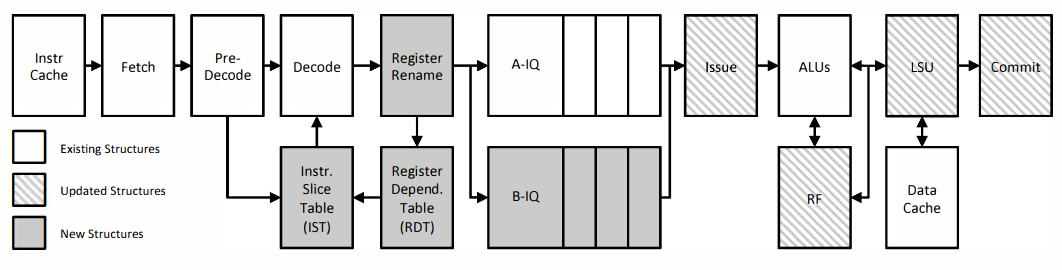
\includegraphics[width=\linewidth]{august22/img/lsc.png}
    \caption{Schematic of the LSC microarchitecture. New structures added to the baseline InO pipeline are shaded gray, while those extended over the baseline InO core are dashed.}
    \end{center}
\end{figure}

\section{Freeflow Core (FC)}

One of the major limitations of the LSC microarchitecture is that the head of the queues of either of the two pipelines may be blocked due to a dependency on a long-latency miss, which stalls the entire processor core. In the LSC microarchitecture, producers of a load in the A-queue may halt execution of younger, ready instructions in the queue depending on where the load is serviced from. Blocking of the A-queue by such instructions keeps execution units idle until their dependencies are resolved. FC identifies these instructions and forwards them to a third in-order queue called the C-queue, which is an alternate execution path for high latency instructions.

FC implements simple 3-bit latency counters, the set counter and the reset counter at the head of queues A and C respectively, in order to keep track of the number of cycles an instruction spends at the head of the queues. In case an instruction stalls the A-queue for more than a fixed number of cycles (chosen as six in the proposed implementation and measured using the set counter), its address is stored in the Freeflow Instruction Slice Table (FIST) and it is forwarded to the C-queue in subsequent executions of the same code. Such instructions are termed high latency instructions. There is also the potentiality that the producer for an instruction that previously stalled the head of the A-queue no longer experiences a long-latency cache miss, and the consuming instruction corresponding to this load now becomes a normal instruction. Hence, if an instruction waits at the head of C-queue for less than a fixed number of cycles (chosen as six in the proposed implementation and measured using the reset counter), the high latency instruction is re-marked as a normal instruction, and its address is invalidated in the FIST.

Experimental analyses conducted show that FC incurs a performance hit of 14\% while being 100\% more power efficient\footnote[2]{Power efficiency is measured in terms of the average number of instructions executed per watt of power spent.} as compared to the OoO design. It performs roughly 89\% better than the InO baseline (as indicated the IPC metric) while being 46\% more power efficient. It outperforms the then state-of-the-art LSC design by 11 percentage points (in terms of IPC).

\begin{figure}[H]
    \begin{center}
    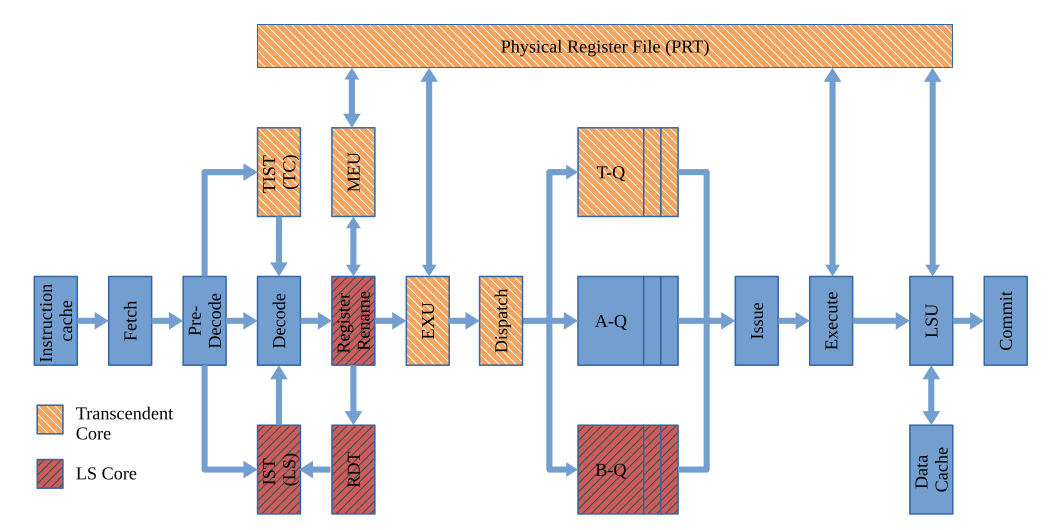
\includegraphics[width=\linewidth]{august22/img/freeflow.png}
    \caption{Schematic of the FC microarchitecture.}
    \end{center}
\end{figure}

\section{Forward Slice Core (FSC)}

The LSC microarchitecture offers limited MHP because of two reasons: (1) the IBDA mechanism needs few iterations to generate backward slices and due to this, during the initial iterations, AGIs are forwarded to the A-queue negatively impacting the exploitable MHP; (2) if the number of AGIs for a particular memory instruction exceeds the finite size of the IST, some of these AGIs won't be accomodated in the IST causing them to be forwarded to the A-queue incorrectly. The LSC microarchitecture also requires additional hardware structures such as the RDT and the IST.

The FSC microarchitecture builds on the basic stall-on-use in-order pipeline. It identifies forward slices corresponding to a load instruction, defined as the sequence of instructions that depend (directly or indirectly) on a previous load instruction. Such forward slice instructions are sent to dedicated in-order queues: execute-type instructions are dispatched to the Dependent Execute Lane (DEL) whereas load-dependent loads are dispatched to the Dependent Load Lane (DLL). Instructions stuck at the head of the DEL for more than a fixed number of cycles (chosen as four in the proposed implementation) are forwarded to the Holding Lane (HL), to pave way for younger ready instructions in the DEL. FSC identifies forward slices dynamically in hardware using the Steering Bit Vector (SBV). SBV has a bit entry corresponding to each physical register. The SBV bit corresponding to the destination physical register of the load instruction encountered first is set. Any younger instruction that consumes a physical register for which the SBV bit is set, the SBV bit corresponding to that instruction's destination register is set. An SBV bit is cleared upon successful computation of the destination physical register corresponding to the instruction that set this bit. This enables FSC to propagate an instruction's dependence on a load forward. Apart from this, for store instructions, the STA micro-op is replicated across all four lanes in order to deal with the memory disambiguation problem. 

\begin{figure}[H]
    \begin{center}
    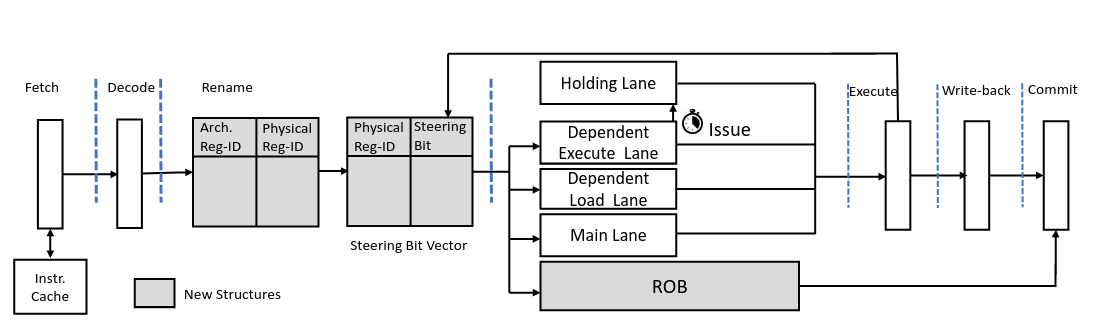
\includegraphics[width=\linewidth]{august22/img/fsc.png}
    \caption{Schematic of the FSC microarchitecture. New structures (apart from the three additional in-order queues) added to the baseline stall-on-use InO pipeline are shaded gray.}
    \end{center}
\end{figure}

Experimental analyses conducted show that the FSC microarchitecture outperforms the InO baseline owing to a 64\% increase in IPC (a gain of 14 percentage points over the then state-of-the-art Freeway\cite{freeway} core), performing within 6.9\% of the OoO core. The area overhead is just 1\% of the baseline InO core, occupying 37\% less chip area compared to the baseline OoO core.

% \chapter{Experiments}
% Hello
% \section{Section}
% Hello \cite{borkar2011future}
% \subsection{SubSection}
% Hello

\chapter{Progress and Future Work}

\section{Completed Work}

\begin{itemize}
    \item Conducted an extensive literature review for restricted OoO microarchitecture proposals.
    \item Installed Sniper multi-core simulator v6.1 and ran multiple experiments and simulations on implementations for \cite{loadslice}, \cite{freeflow} and \cite{forwardslice}.
\end{itemize}

\section{Plans for September}

\begin{itemize}
    \item Debugging incorrect project implementation for \cite{forwardslice}.
    \item Reading and reviewing work done in \cite{fxa}, and going through its implementation.
    \item Reading and reviewing work done for fault-tolerant architectures in \cite{remo} and \cite{remora}.
\end{itemize}

\bibliographystyle{ieeetr}
\bibliography{thesisTemplate}{}
\end{document}